%%%%%%%%%%%%%%%%%%%%%%%%%%%%%%%%%%%%%%%%%%%%%%%%%%%%%%%%%%%%%%%%%
%%%  ISWC 2016 Demo:   %%%%
%%%%%%%%%%%%%%%%%%%%%%%%%%%%%%%%%%%%%%%%%%%%%%%%%%%%%%%%%%%%%%%%%

\documentclass[runningheads,a4paper]{llncs}
\usepackage{graphicx}
\usepackage{amsmath}
\usepackage{todonotes}
\usepackage{hyperref}
\usepackage{amssymb, bm}
\usepackage{indentfirst}

%%%%%%%%%%%%%%%%%%%%%%%%%%%%%%%
%%%  Beginning of document  %%%
%%%%%%%%%%%%%%%%%%%%%%%%%%%%%%%

\begin{document}

\title{A title}

\titlerunning{A title}

\author{Manel Achichi$^1$, Pasquale Lisena$^2$, Eva Fern\'{a}ndez$^2$, Wafa Bouneb$^2$, \\ Konstantin Todorov$^1$, Rapha\"{e}l Troncy$^2$}
\authorrunning{Achichi, Lisena \textit{et al.}}
\institute{$^1$University of Montpellier, France\\ $^2$EURECOM, Sophia Antipolis, France}

\maketitle

%%%%%%%%%%%%%%%%%%
%%%  Abstract  %%%
%%%%%%%%%%%%%%%%%%

\begin{abstract}
In this paper, we introduce OVERTURE---an application allowing to explore the catalogs of major music bibliographic agencies, including the French National Library, Radio France and the Philharmonie de Paris. The application is based on the {\it marc2rdf} prototype, developed for this purpose and allowing for the conversion of bibliographical entries about music works, interpretations and expressions from their original MARC-format to RDF, following the DOREMUS model, an extension of the well-known FRBRoo model.
\end{abstract}

%%%%%%%%%%%%%%%%%%%%%%%%%
%%%  1. Introduction  %%%
%%%%%%%%%%%%%%%%%%%%%%%%%

\section{Introduction}
\label{sec:introduction}

-- The Doremus project: talk about the model \ref{} and the controlled vocabularies \ref{} because we need this info in next section, cite the doremus poster paper \cite{achichi2015doremus}

-- the input data,

-- why it is important to convert these data to RDF (impact, number of institutions using this format).

%%%%%%%%%%%%%%%%%%%%%%%%%%%%%%%%%%%%%%%%%%%%%
%%%  2. Converting Music Metadata to RDF  %%%
%%%%%%%%%%%%%%%%%%%%%%%%%%%%%%%%%%%%%%%%%%%%%

\section{Converting Music Metadata to RDF}
\label{sec:conversion}

\section{Converting Music Metadata to RDF}
\label{sec:conversion}
The data collected from the BnF and the Philharmonie de Paris (PP) describing music works are given in the MARC format, and more precisely, its UNIMARC and INTERMARC variants. A MARC file is a succession of fields, each carrying a label (a three-digit number) and subfields, delimited by the \$ symbol, as shown in Fig.~\ref{fig:unimarc}. The semantics of these fields and subfields is described in various documents issued by The International Federation of Library Associations and Institutions (IFLA)\footnote{\url{http://www.ifla.org/publications/ifla-series-on-bibliographic-control-36}.}. %, according to the MARC variant. 
Note that a subfield tag can change its meaning depending on the field under which it is found. In the example in Fig.~\ref{fig:unimarc}, the combination of the field 500 with the \$a tag stands for the musical genre (sonata in this case), whereas the same tag under the field 700 stands for the composer name (Beethoven).

\begin{figure}
  \centering
  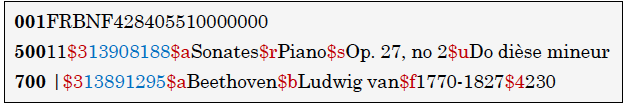
\includegraphics[width=8cm]{img/marc-exmpl-simple.png}
  \caption{An excerpt of a UNIMARC record.}
  \label{fig:unimarc}
\end{figure}

We have developed an open source prototype that allows for the automatic conversion of bibliographic records given in UNI- or INTERMARC to RDF\footnote{\url{https://github.com/DOREMUS-ANR/marc2rdf}}, implementing the DOREMUS model. The conversion process relies on explicit expert-defined transfer rules (or mappings) that indicate where in the MARC file to look for what kind of information, providing its corresponding property path in the model as well as useful examples that illustrate each transfer rule, as shown in Fig.~\ref{fig:mappings}. %The mapping rules reflect the practices of each institution and therefore a mapping table per institution has been provided by the experts. 
We have used the DOREMUS properties to name the extracted relations (as for example \texttt{mus:U12$\_$has$\_$genre}\footnote{The \texttt{mus} prefix refers to \url{http://data.deremus.org/ontology/}}, labeling the property describing the genre of a work). The resources are identified by URIs that use the corresponding DOREMUS class labels in their names (as for example \url{http://data/doremus.org/expression/UUID} identifying uniquely an instance of the FRBRoo class \texttt{Expression}).

\begin{figure}
  \centering
  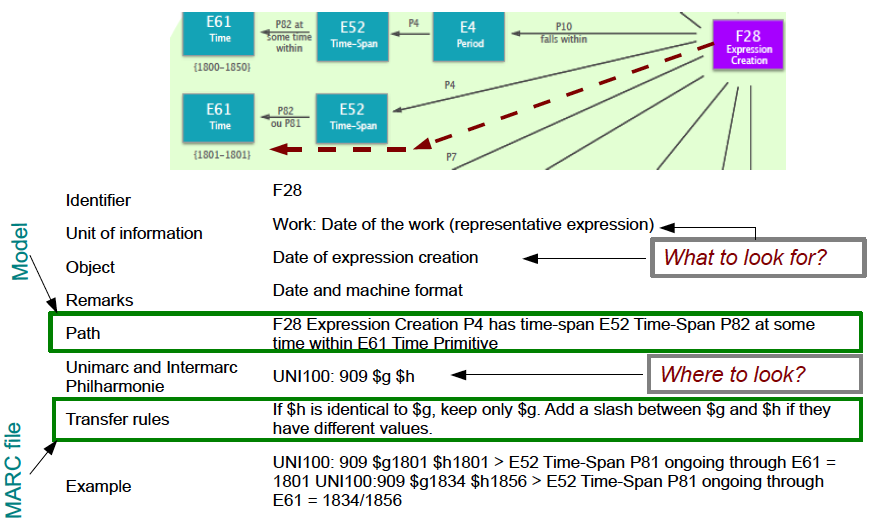
\includegraphics[width=11cm]{img/mapping-rules.png}
  \caption{Example of mapping rules regarding the timespan of the composition of a work.}
  \label{fig:mappings}
\end{figure}

Often, the RDF data that we extract will contain string literal values, such as genres ({\it sonata}) or instruments ({\it piano}). These values are controlled by specific vocabularies, such as the MIMO vocabulary\footnote{\url{http://www.mimo-international.com/vocabulary.html}} describing musical instruments. Therefore, our data conversion methods include an automatic mapping of string literals to URIs coming from controlled vocabularies. Inspired by the Datalift platform~\cite{datalift}, we have developed a generic \texttt{string2uri} component enabling to lookup strings in a SKOS controlled vocabulary and to propose best candidate match.
%An example of a converted MARC record is given in Fig. \ref{}. %Not sure we need an example.

%%%%%%%%%%%%%%%%%%%%%%%%%%%%%%%%%%%%%%%%%%%%%%%%%%%%%%%%%%%%%
%%%  3.Data linking  %%%
%%%%%%%%%%%%%%%%%%%%%%%%%%%%%%%%%%%%%%%%%%%%%%%%%%%%%%%%%%%%%

\section{Data Heterogeneities and Linking}

Due to the high data heterogeneity, link discovery in the musical field becomes a challenging task. To train and test data linking tools, we have collected benchmark data from the BnF and the PP, now part of the OAEI instance matching evaluation campagne\footnote{\url{http://islab.di.unimi.it/content/im_oaei/2016/#doremus}}. Our tests with  SILK \cite{jentzsch2010silk} and LIMES \cite{ngomo2011limes}, achieving an average F-measure of around 55\%, confirm that new methods, specific to the music field, need to be proposed, in order to handle specific heterogeneity types of these datasets. In particular, special attention has to be payed to multilingual descriptions of works, as well as to significant lexical differences in work titles. Descriptive heterogeneities (level of detail, number of properties) also hinder the performance of general purpose tools. Furthermore, certain properties, although mapped correctly according to the transfer rules, contain highly heterogeneous information, as for example \texttt{cidoc-crm:P3$\_$has$\_$note} -- a field of free text in the form of comments. We are currently developing a linking approach that combines expert heuristics with indexing techniques that is able to propose a solution according to the heterogeneity type manifested by the data.
%%%%%%%%%%%%%%%%%%%%%%%%%%%%%%%%%%%%%%%%%%%%%%%%%%%%%%%%%%%%%
%%%  3. OVERTURE: an Exploratory Search Engine for Music  %%%
%%%%%%%%%%%%%%%%%%%%%%%%%%%%%%%%%%%%%%%%%%%%%%%%%%%%%%%%%%%%%

\section{OVERTURE: an Exploratory Search Engine for Music}
\label{sec:overture}
\begin{figure}
  \centering
  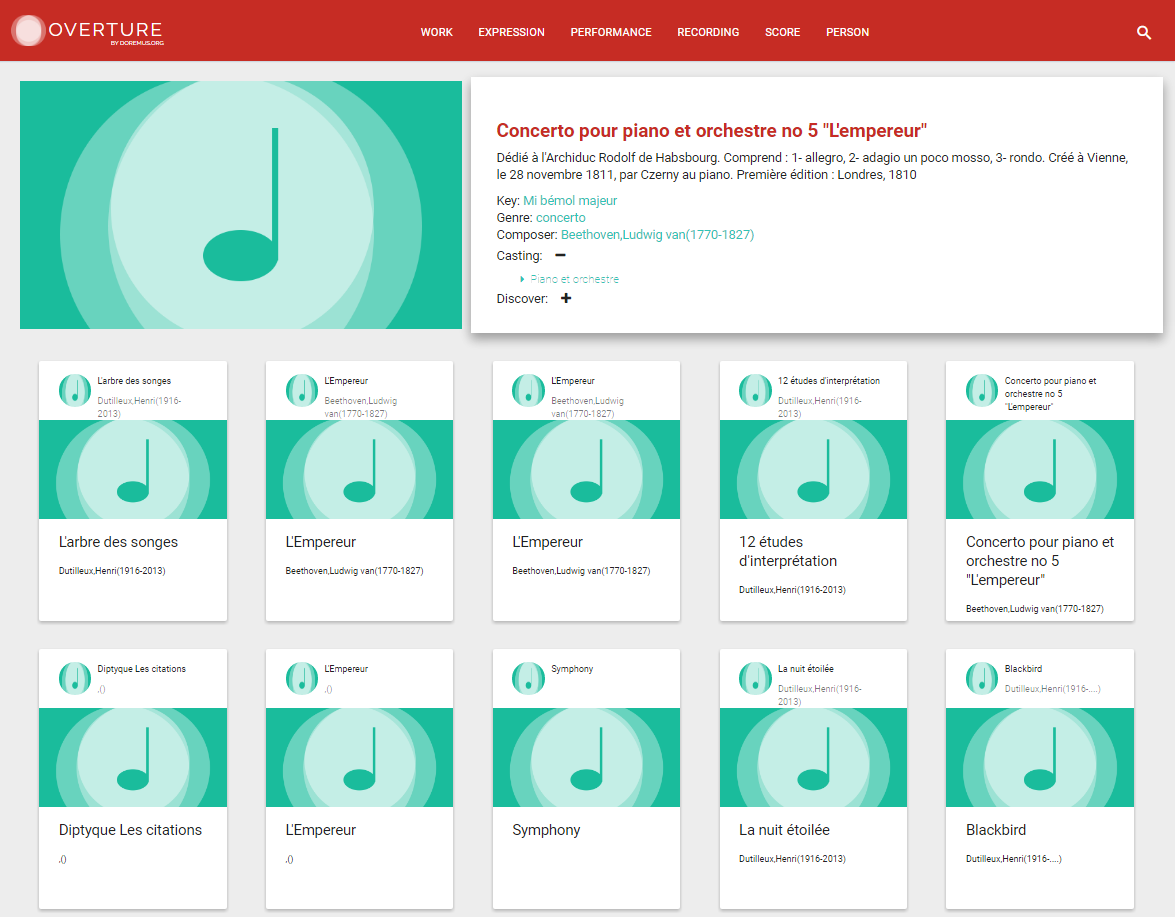
\includegraphics[width=11cm]{img/overture-detail.png}
  \caption{Overture: Browsing Expression ...}
  \label{fig:overture-detail}
\end{figure}

OVERTURE (Ontology-driVen Exploration and Recommendation of mUsical REcords) is a modern web application that relied on a Node.JS server sitting in front of a Virtuoso triple store where all the data has been loaded. The web application performs SPARQL queries to access the data. Figure~\ref{fig:overture-detail} shows the user interface realized with AngularJS. On top, a navigation bar directs the user towards one of the main concepts in the DOREMUS model (Work, Expression, Performance, Recording, Score, Person), that become distinct sections of the application. Inside each section, the user can filter the list of records shown in a class-specific and advanced search form. In this way, (s)he can search a performance by choosing a particular location, a performer, or an expression by selecting the musical key, the genre or by searching by title. From these parameters, the server generates the SPARQL query that matches the user information need (Figure~\ref{fig:sparql}).

Clicking on a result, more details are shown like the information about the composer, the casting and a longer descriptive note. Beside it, a selection of different expressions is shown. In the future, this selection will contain related expressions, selected through a recommendation algorithm.
\begin{figure}
\centering
\begin{verbatim}
SELECT ?expressions ?title
WHERE {
    ?expressions a frbroo:F22_Self-Contained_Expression ;
        cidoc:P102_has_title ?title .
        mus:U12_has_genre <http://data.doremus.org/vocabulary/genre/si>
}
\end{verbatim}
\caption{Overture: A simplified example of the SPARQL query that extracts the titles of expressions that have the genre "symphony".}
\label{fig:sparql}
\end{figure}

% TODO link to demo video

%%%%%%%%%%%%%%%%%%%%%%%%%%%%%%%%%%%%%%%
%%%  4. Conclusion and Future Work  %%%
%%%%%%%%%%%%%%%%%%%%%%%%%%%%%%%%%%%%%%%

\section{Conclusion and Future Work}
\label{sec:conclusion}


%We are currently working on the development of connectors for music works, allowing for the automatic interlinking of equivalent resources across datasets of different bibliographical agencies. Our first test with the SILK \cite{jentzsch2010silk} and LIMES \cite{ngomo2011limes} tools confirm our initial hypothesis that new methods, specific to the music field, need to be proposed, in order to handle the high heterogeneity of these datasets. In particular, our first tests show that special attention has to be payed to multilingual descriptions of works, as well as to significant differences in lexical descriptions of music titles. Descriptive heterogeneities (level of detail, amount of information available) also appear to be hard to handle by the existing general purpose off-the-shelf linking tools. We plan to combine expert heuristics with an automatic heterogeneity centered data linking approach. Finally, the developed connectors will be integrated to the OVERTURE application, allowing for the automatic navigation from one dataset to another bringing to the user the richness of several connected datasets.

%Recommendation ?

\section*{Acknowledgments}
This work has been partially supported by the French National Research Agency (ANR) within the DOREMUS Project, under grant number ANR-14-CE24-0020.

\bibliographystyle{abbrv}
\bibliography{bib-doremus}

\end{document}
